\documentclass{report}
\usepackage[T1]{fontenc} % Fontes T1
\usepackage[utf8]{inputenc} % Input UTF8
\usepackage{csquotes}
\usepackage[portuguese]{babel} %Usar língua portuguesa
\usepackage{blindtext} % Gerar texto automaticamente
\usepackage[printonlyused]{acronym}
\usepackage{hyperref} % para autoref
\usepackage{graphicx}
\usepackage{url}
\usepackage{float}
\usepackage{placeins}
\usepackage[backend=biber, style=ieee]{biblatex} % para usar bibliografia
\usepackage[portuguese]{babel} %Usar língua portuguesa
\usepackage{subcaption}


\begin{document}
%%
% Definições
%
\def\titulo{Projeto 2}
\def\data{Junho 2020}
\def\autores{André Silva, André Alves, Rafael Santos, Leonardo Francisco}
\def\autorescontactos{(98651) andrecastrosilva@ua.pt, (98466) rafaelmsantos@ua.pt, (94190) afla@ua.pt, (97772) l.fiuza@ua.pt }
\def\departamento{DETI}
\def\empresa{Universidade de Aveiro}
\def\logotipo{ua.png}
%
%%%%%% CAPA %%%%%%
%
\begin{titlepage}

\begin{center}
%
\vspace*{50mm}
%
{\Huge \titulo}\\ 
%
\vspace{10mm}
%
{\Large \empresa}\\
%
\vspace{10mm}
%
{\LARGE \autores}\\ 
%
\vspace{30mm}
%
\begin{figure}[h]
\center
\includegraphics{\logotipo}
\end{figure}
%
\vspace{30mm}
\end{center}
%
\end{titlepage}

%%  Página de Título %%
\title{%
{\Huge\textbf{\titulo}}\\
{\Large \departamento\\ \empresa}
}
%

\author{
(98651) andrecastrosilva@ua.pt, (98466) rafaelmsantos@ua.pt, \\ (94190) afla@ua.pt, (97772) l.fiuza@ua.pt
}
%
\date{\data}
%
\maketitle

\pagenumbering{arabic}

%%%%%% RESUMO %%%%%%
\begin{abstract}
\par O objetivo deste projeto consistiu na criação de um sistema que permita inserir, visualizar e comentar imagens enviadas para uma aplicação, replicando funcionalidades que se ecnontram noutros serviços. \par


\end{abstract}

%%%%%% Agradecimentos %%%%%%
\renewcommand{\abstractname}{Agradecimentos}
\begin{abstract}
\par Queremos agradecer aos nosso professores da unidade curricular de Laboratórios de Informática, André Ventura Zúquete, António Manuel Adrego da Rocha, João Paulo Barraca por nos ter guiado durante o projeto e incentivado a realizá-lo da melhor forma possível. Aprendemos mais um bocado sobre cada matéria à medida que fomos avançando no trabalho, demonstrando assim que este último trabalho prático é indispensável na cadeira de LABI.

\end{abstract}


\tableofcontents
% \listoftables     % descomentar se necessário
% \listoffigures    % descomentar se necessário


%%%%%%%%%%%%%%%%%%%%%%%%%%%%%%%
\clearpage
\pagenumbering{arabic}

%%%%%%%%%%%%%%%%%%%%%%%%%%%%%%%%
\chapter{Introdução}
\label{chap.introducao}

\par
Este relatório aborda a maneira . Este documento está dividido em 4 capítulos principais, no \autoref{chap.2} é onde se fornece o único interface para interação com o sistema. No \autoref{chap.3} é onde apresentamos métodos que permitem a navegação entre os diversos componentes. O \autoref{chap.4} é composto por métodos que permitem o registo de informação numa base de dados relacional e a obtenção de informação da mesma. O \autoref{chap.5} que se executa como parte da Aplicação Web, é onde terá métodos para lidar com imagens enviadas para o sistema, ou a obtenção das mesmas.  \par 
Finalmente, no \autoref{chap.6} são apresentadas as conclusões retiradas do trabalho.

\chapter{Interface Web}
\label{chap.2}

\section{Páginas Criadas}
\par 
No que toca à interface web foi usada uma template Ratchet( acessível em \href{http://goratchet.com/components/}{Ratchet Components}).\par
\par
O que é o Ratchet? O Ratchet é uma framework com HTML, CSS e JavaScript permitindo criar páginas web que podem ser adaptadas a vários aparelhos diferentes.
\par
Foram criadas 5 páginas html : uma Home , uma onde teria o feed de imagens , uma onde era possível publicar uma imagem, uma onde era possível ver o perfil da pessoa e por fim uma que fala do projeto e dos seus criadores.


\begin{figure}[hbt!]
\centering
\begin{subfigure}{.5\textwidth}
  \centering
  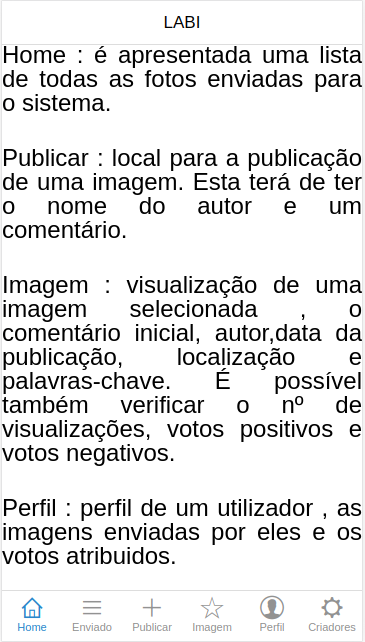
\includegraphics[width=0.6\linewidth]{home.png}
  \caption{}
\end{subfigure}%
\begin{subfigure}{.5\textwidth}
  \centering
  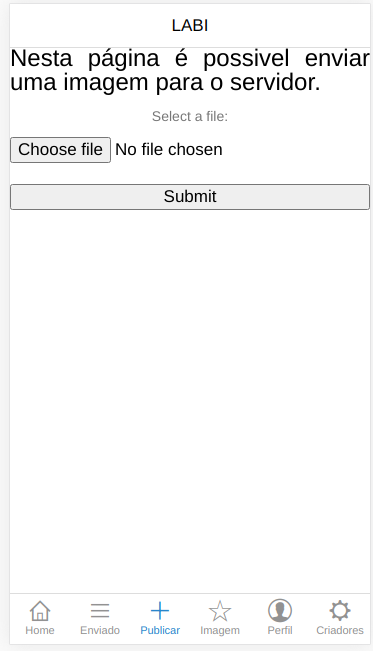
\includegraphics[width=0.6\linewidth]{publicar.png}
  \caption{}
\end{subfigure}
\begin{subfigure}{.5\textwidth}
  \centering
  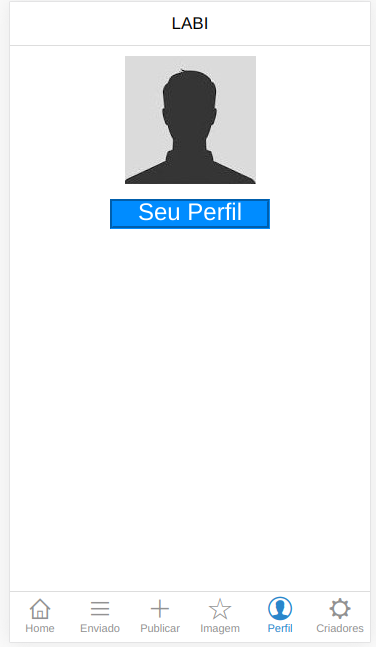
\includegraphics[width=0.6\linewidth]{perfil.png}
  \caption{}
\end{subfigure}%
\begin{subfigure}{.5\textwidth}
  \centering
  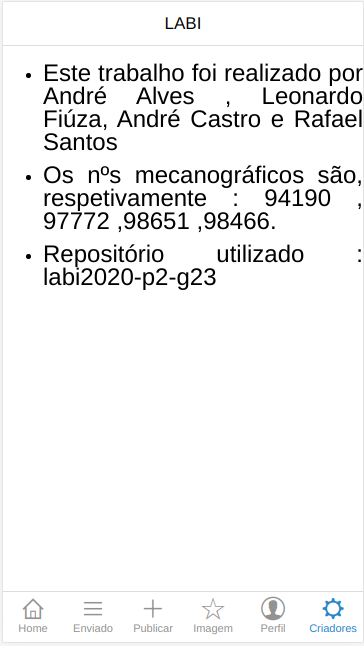
\includegraphics[width=0.6\linewidth]{criadores.png}
  \caption{}
\end{subfigure}%
	\caption{Todas as páginas a funcionar, menos a Perfil e a Publicar.}
\end{figure}




\clearpage

\chapter{Aplicação Web}
\label{chap.3}
\par 
Para interligar as páginas e para que a aplicação funcionasse corretamente foi necessário utilizar uma framework.
\par 
Uma framework é um conjunto de código escrito que procura aumentar a eficiência do programador ao oferecer-lhe funções e funcionalidades de modo a que o programador não esteja constantemente a reescreve-la para cada aplicação.
\par
A framework utilizada neste projeto foi o cherrypy que não só serviu como framework como também funcionou como servidor web.

\begin{figure}[h]
\begin{center}
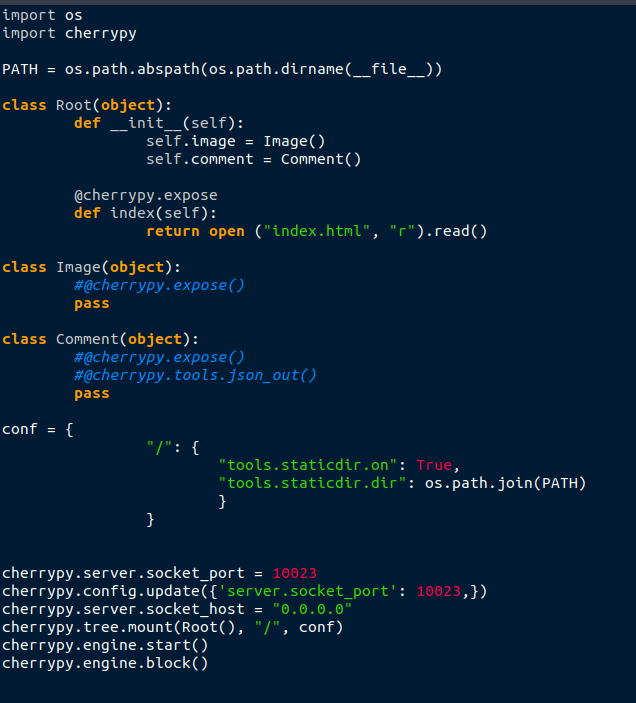
\includegraphics[width = 5cm, height= 7cm]{app.png}
  \caption{Código aplicação}
  \label{fig:boat1}
\end{center}
  
\end{figure}


\chapter{Persistência}
\label{chap.4}
\section{Base de dados}
\par A base de dados tem como objetivo o armazenamento de diversos tipos de informação relacionada, de tal forma que a sua atualização e consulta possa ser eficiente e efetuada num curto espaço de tempo e para facilitar a oranização, manutenção e pesquisa de dados. \par

%%Figura Declaration
\FloatBarrier
\begin{figure}[H]
    %\centering
    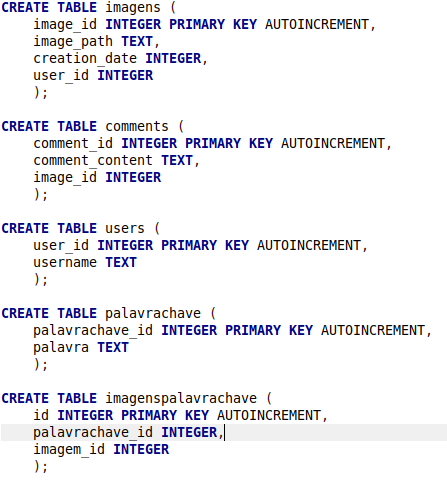
\includegraphics[scale=0.5]{basededados.png}
    \caption{Esqueleto base de dados}
    \label{fig:my_label}
\end{figure}

\chapter{Processador de imagens}
\label{chap.5}
\par
No que toca ao processamento de imagens tivemos algumas dificuldades no envio da fotos para o sistema e no tratamento das mesmas.
\par
Conseguimos realizar os efeitos , no entanto também não o conseguimos aplicar sendo o passo anterior necessário.Apesar disto , testamos os efeitos com imagens do nosso portátil e estão totalmente funcionáveis.
\begin{figure}[hbt!]
\centering
\begin{subfigure}{.5\textwidth}
  \centering
  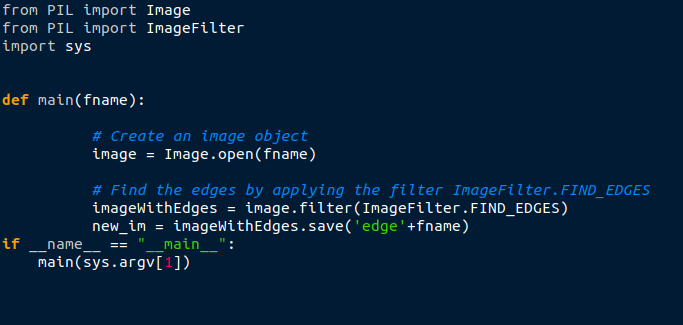
\includegraphics[width=0.8\linewidth]{edge.png}
  \caption{Efeito edge}
\end{subfigure}%
\begin{subfigure}{.5\textwidth}
  \centering
  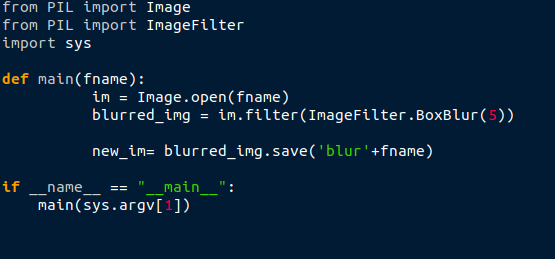
\includegraphics[width=0.8\linewidth]{blur.png}
  \caption{Efeito blur}
\end{subfigure}
\begin{subfigure}{.5\textwidth}
  \centering
  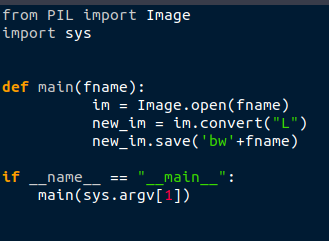
\includegraphics[width=0.8\linewidth]{bandw.png}
  \caption{Efeito preto e branco}
\end{subfigure}
\end{figure}





\chapter{Conclusões}
\label{chap.6}
\par 
Apesar de não termos realizado o projeto na integra consideramos que este projeto nos ajudou a desenvolver capacidades e competências na área do desenvolvimento das aplicações web, manipulção de dados e base de dados.
Concluindo , sabemos que não atingimos todos os objetivos mas enriqueceu o nosso percurso académico.
\chapter*{Contribuições dos autores}
\par Consideramos que houve uma participação de 25\% atribuída a cada um dos autores. 

\end{document}